\begin{enumerate}
\item {\bf (8 points)} Build a 4-bit universal shift register in
Table~\ref{table:uni} using D flip-flops and 8:1 multiplexers.

\begin{table}
\begin{tabular}{c|c|c||c}
S2 & S1 & S0 & Operation \\ \hline
0  &  0 &  0 & Hold \\ \hline
0  &  0 &  1 & Load \\ \hline
0  &  1 &  0 & ASR  \\ \hline
0  &  1 &  1 & ASL  \\ \hline
1  &  0 &  0 & LSR  \\ \hline
1  &  0 &  1 & LSL  \\ \hline
1  &  1 &  0 & CSR  \\ \hline
1  &  1 &  1 & CSL  \\ 
\end{tabular}
\caption{The truth table for a universal shift register.}
\label{table:uni}
\end{table}

\begin{solution}{
\begin{figure}[ht]
\center{
\includegraphics{./FigHw6/Prob6-1}}
\end{figure}
}\end{solution}

\item {\bf (8 pts.)} Use a counter and a comparator
to implement the following circuits.

\begin{enumerate}
\item Show how to modify the counter (by adding some external logic)
to implement a mod-10 counter.  A mod-10 counter counts from 0 to
9 and then goes back to 0.  It spends one full clock cycle on each
of these count values.

\begin{solution}{
Our mod 10 counter will have 1 data input, representing
the state of the least significant counter.  Call this input
Nine In.  Nine In equals 1 when the less significant counters
output equals 9, otherwise Nine In equals 0.  Our mod 10 counter
will have four bits of output representing the current count value.
The mod 10 counter will also have a Nine Out output which will
equal 1 when our current count value equals 9, otherwise
Nine Out equals 0.  Let the constant value 9 be sent to the Y
input of the comparator and the 4-bit register (Q) sent to the X
input.  When Q<9 the comparator outputs G=0, L=1, E=0.  When
Q=0 then the comparator outputs G=0, L=0, E=1.  Hence by running
the E output of the comparator to the select input of the mux,
the Q+1 will be sent to the register input when Q<9.  Notice
that the register will only latch a new value (Q+1 or 0) when
the less significant counter has rolled over.

\begin{figure}[ht]
\center{
\includegraphics{./FigHw6/Prob6-2}}
\end{figure}

}\end{solution}

\item Use four mod-10 counters to build a 4-digit decimal counter which 
counts up from 0 to 9999.  Draw a schematic for the 4-digit decimal 
counter. 
\begin{solution} {
Just ripple four of the above counter head to tail via Nine In and Nine
Out.  Set the Nine In input of the least significant counter to 1.
} \end{solution}

\end{enumerate}


\item {\bf (8 pts.)} Design a circuit which contains three 8-bit 
registers X,Y,Z.  The behavior of the circuit is determined by the statement:
\begin{verbatim}
if (X > Y) then Z = X+X else Z = Y+Y
\end{verbatim}
The registers are preloaded with values in them.
Submit a circuit diagram showing the building blocks uses,
their interconnections and any miscellaneous logic required to make
them operate together.
\begin{solution} {
\begin{figure}[ht]
\center{
\includegraphics{./FigHw6/Prob6-3}}
\end{figure}
} \end{solution}


\item {\bf (8 pts.)} Design a circuit which contains three registers X,Y,Z.
The behavior of the circuit is determined by the statements:
\begin{verbatim}
1. while (X > 0) {
2.     Z = Z+Y;
3.     X = X-1;
4. } 
\end{verbatim}
The registers are preloaded with values in them.
Submit a circuit diagram showing the building blocks used,
their interconnections and any miscellaneous logic required to make
them operate together.  The design should use an adder and an
adder subtractor plus some other building blocks.  Hint, use
the enable inputs of the registers to control when they
latch information.

\begin{solution} {
\begin{figure}[ht]
\center{
\includegraphics{./FigHw6/Prob6-4}}
\end{figure}
} \end{solution}

\item {\bf (8 pts.)} Given three 32-bit registers A,B,PC, design a circuit
which adds PC and A (putting the result back into PC) when A is equal
to B.  Otherwise, add 1 to PC.  The contents of A and B
are to remain unchanged.

\begin{solution} {
\begin{figure}[ht]
\center{
\includegraphics{./FigHw6/Prob6-5}}
\end{figure}
} \end{solution}

\item {\bf (8 pts.)} Build a circuit that performs the following: 
\begin{verbatim}
    for(i=0; i<100; i++) 
        total = total + i;
\end{verbatim}
Use the counter described in this chapter for the $i$ variable; 
assume that the counter is initialized to 0. \verb^total^ is stored 
in a register and its initialized to 0.  Use a comparator to shut 
down the counter and put the register in hold when the count value 
reaches a critical value. Until this critical value is 
reached the comparator should allow the counter to count and the 
register to load.  

\begin{solution} {
Note that the counter really needs only one of two control settings
00 for holding and 10 for counting up.  Thus, the LSB of the counters
control input can be hardwired to 0.  Its the MSB of the counters control
that needs controlled by the comparator.  Since the counter is in the
range of 0-100, the counter has a 7-bit output.  It is an interesting exercise to
determine the number of bits required for the adder's output so that it 
does not overflow during the computation.  The figure below shows that
13 bits are required (the upper six bits of the counter's output are padded
with 0's so that the counters output can be feed into the adder).

\begin{figure}[ht]
\center{
\includegraphics{./FigHw6/Prob6-6}}
\end{figure}
} \end{solution}


\item{\bf (8 pts.)} Build a circuit that performs the following: 
\begin{verbatim}
    for(i=0; i<100; i++) 
        total = total + 1;
\end{verbatim}

\begin{solution} {
\begin{figure}[ht]
\center{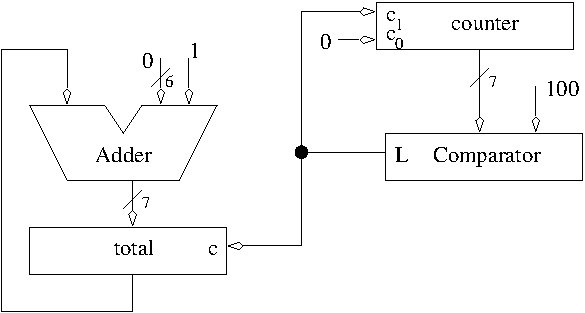
\includegraphics{./FigHw6/Prob6-7}}
\end{figure}
} \end{solution}


\item{\bf (8 pts.)} Design a circuit that can shift (circular 
to the right) the contents of register X by an amount given in 
register Y. X is stored in the circular shift register described 
in this chapter. The solution will require a comparator and a
counter.
\begin{solution} {
\begin{figure}[ht]
\center{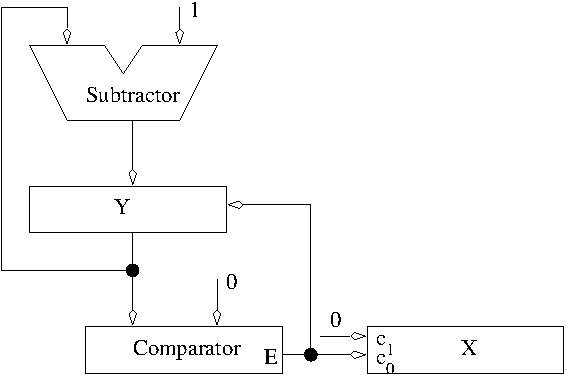
\includegraphics{./FigHw6/Prob6-8}}
\end{figure}
} \end{solution}


\item{\bf (8 pts.)} Assume a 32kx8 RAM is full of data. Show 
the hardware required to realize the following algorithm. 
\begin{verbatim}
    for(i=0; i<32767; i++)
        total = total + M[i];
\end{verbatim}

Where \verb+M[i]+ is the 8-bit word stored at address \verb^i^. 
Assume the total register is initialized to 0. The $i$ variable should 
be the output of a counter. Use a comparator to shut down the counter 
and to put the register in hold when the count value reaches a critical 
value.  
\begin{solution} {
\begin{figure}[ht]
\center{
\includegraphics{./FigHw6/Prob6-9}}
\end{figure}
} \end{solution}


\item{\bf (8 pts.)} Show how to initialize a 32kx8 RAM in the following manner. 
\begin{verbatim}
    for(i=0; i<32767; i++) 
        M[i] = i mod 256;
\end{verbatim}

Where the ``i mod 256" statement means store the least significant 
eight bits of the $i$ variable into the RAM. 

\begin{solution} {
\begin{figure}[ht]
\center{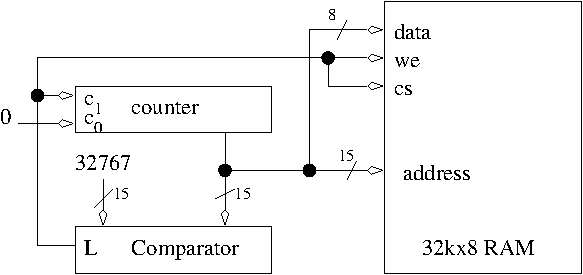
\includegraphics{./FigHw6/Prob6-10}}
\end{figure}
}\end{solution}

\item{\bf (5 pts.)} Complete the timing diagram in Figure~\ref{fig:hwshift}
\label{item:shifter}
for a 4-bit arithmetic shift register.  Use the control setting from the
truth table on page~\pageref{page:shi}.
\begin{figure}[ht]
\center{
\includegraphics{./FigHw6/Prob6-14}}
\caption{The timing diagram for a 4-bit arithmetic shift register in 
Problem~\ref{item:shifter}.}
\label{fig:hwshift}
\end{figure}

\begin{solution} {
\begin{figure}[ht]
\center{
\includegraphics{./FigHw6/Prob6-13}}
\end{figure}
} \end{solution}


\item{\bf (5 pts.)} Complete the timing diagram in Figure~\ref{fig:hwcount}
\label{item:counter}
for a 4-bit counter.  Use the control setting from the truth table on 
page~\pageref{page:counter}.
\begin{figure}[ht]
\center{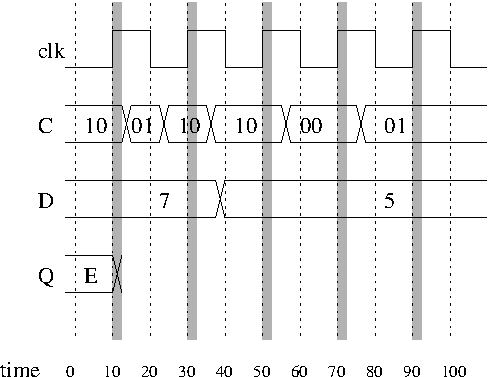
\includegraphics{./FigHw6/Prob6-15}}
\caption{The timing diagram for a 4-bit counter in 
Problem~\ref{item:counter}.}
\label{fig:hwcount}
\end{figure}

\begin{solution} {
\begin{figure}[ht]
\center{
\includegraphics{./FigHw6/Prob6-14}}
\end{figure}
} \end{solution}


\item{\bf (5 pts.)} Complete the timing waveforms for $A_1, A_0, Q_1, Q_0$
\label{item:cascade}
based on the circuit diagram shown in Figure~\ref{fig:cascade}.  Use the truth 
table on page~\pageref{page:reg} for the register. Put the decimal 
representation of the signals in the timing diagram (like the timing 
diagram in Figure~\ref{fig:comb1}).
\begin{figure}[ht]
\center{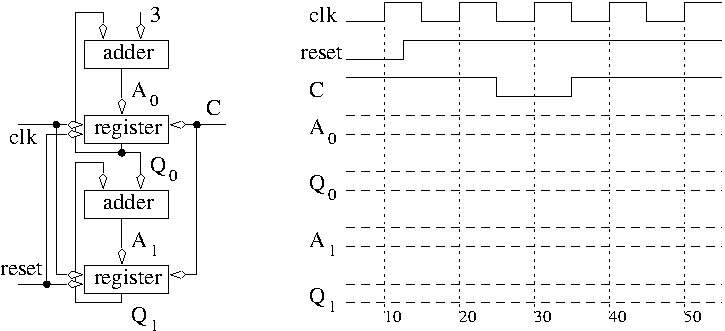
\includegraphics{./FigHw6/Prob6-16}}
\caption{The circuit diagram and incomplete timing diagram for 
Problem~\ref{item:cascade}.}
\label{fig:cascade}
\end{figure}

\begin{solution} {
\begin{figure}[ht]
\center{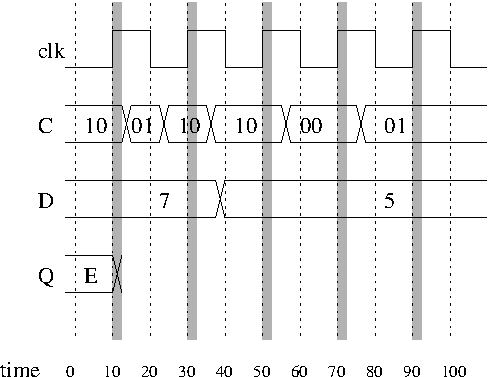
\includegraphics{./FigHw6/Prob6-15}}
\end{figure}
} \end{solution}

\item{\bf (4 pts.)} The circuit shown in Figure~\ref{fig:fib} generates a
Fibonacci sequence, a sequence starting with 1,1,2,3...  The next number in
the sequence is the sum of the preceding two numbers.  Complete the 
timing diagram, assuming the circuit starts with the values shown.
Identify the signal which generates a complete Fibonacci sequence.

\begin{figure}[ht]
\center{
\includegraphics{./FigHw6/fib}}
\caption{A circuit which generates a Fibonacci sequence.}
\label{fig:fib}
\end{figure}

\end{enumerate}
